\section{E-Mail Verschlüsselung}

\frame{%
  \frametitle{Inhaltsverzeichnis}
  \tableofcontents[currentsection]
}

\begin{frame}
  \frametitle{Probleme symmetrischer Verschlüsselung}
  \begin{itemize}
    \item Verteilung der Schlüssel
    \item Anzahl benötigter Schlüssel
    \pause
    \begin{itemize}
      \item 2 Personen $\rightarrow$ 1 Schlüssel
      \item 3 Personen $\rightarrow$ 3 Schlüssel
      \item 4 Personen $\rightarrow$ 6 Schlüssel
      \item 100 Personen $\rightarrow$ 4950 Schlüssel
      \item n Personen $\rightarrow$ $\frac{n(n-1)}{2}$ Schlüssel
    \end{itemize}
    \todo[inline]{Evtl auf Tafel rechnen}
    \todo[inline]{Graph}
  \end{itemize}

\end{frame}

\begin{frame}
  \frametitle{Asymmetrische Verschlüsselung}
  \framesubtitle{Grundlagen}
  \begin{columns}[c]
    \begin{column}{0.5\textwidth}
      \center \inputSVG[\def\svgscale{0.2}]{Orange_blue_public_private_keygeneration_de}
    \end{column}
    \begin{column}{0.5\textwidth}
      \center \inputSVG[\def\svgscale{0.2}]{Orange_blue_public_key_cryptography_de}
    \end{column}
  \end{columns}
\end{frame}

\begin{frame}
  \frametitle{Asymmetrische Verschlüsselung}
  \framesubtitle{Schema}
  \center \inputSVG[\def\svgscale{0.2}]{Orange_blue_public_key_scheme_de}
\end{frame}

\begin{frame}
  \frametitle{Schlüsselserver (Keyserver)}
  \center \inputSVG[\def\svgscale{0.2}]{Orange_blue_keyserver_de}
\end{frame}

\begin{frame}
  \frametitle{Identitätsprüfung}
  \begin{itemize}
    \item Keine Echtheitsgarantie für Schlüssel auf Schlüsselserver
    \item ``Web of Trust''
    \note{Schlüssel nur signieren wenn WIRKLICH geprüft}
  \end{itemize}
  \center \inputSVG[\def\svgscale{0.2}]{Orange_blue_web_of_trust_de}
\end{frame}

\begin{frame}
  \frametitle{Signaturen}
  \center \inputSVG[\def\svgscale{0.2}]{Orange_blue_digital_signature_de}
  \todo[inline]{Schaubild Signaturschema}
\end{frame}

\begin{frame}
  \frametitle{Signierte E-Mail}
  \begin{itemize}
    \item Garantiert Echtheit des Absenders
    \item Keine Verschlüsselung!
    \note{Unterschriebener Vertrag}
    \item Kann aber mit Verschlüsselung kombiniert werden
  \end{itemize}
\end{frame}

\begin{frame}
  \frametitle{Wie kann ich E-Mail Verschlüsselung verwenden?}
  \begin{columns}[c]
    \begin{column}{0.5\textwidth}
      \begin{itemize}
        \item OpenPGP
        \item Phil Zimmermann (1991)
        \item Integration in E-Mail Client
        \begin{itemize}
          \item Thunderbird: Enigmail
          \item Mail: GPGTools
          \item Outlook: ---
        \end{itemize}
      \end{itemize}
      \center 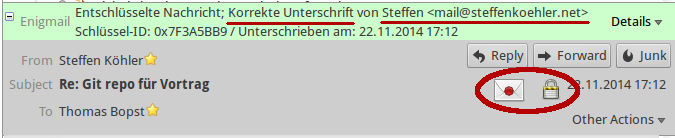
\includegraphics[width=\textwidth]{Enigmail-Screenshot}\\
      \todo{Screenshot für Apfeltool}
    \end{column}
    \begin{column}{0.5\textwidth}
          Konfiguration:
      \begin{enumerate}
        \item Schlüsselpaar generieren
        \item Widerrufszertifikat erzeugen
        \item Öffentlichen Schlüssel auf Schlüsselserver laden
        \item Öffentliche Schlüssel von Freunden/Kollegen \ldots{} herunterladen
      \end{enumerate}
    \end{column}
  \end{columns}

\end{frame}
